% Options for packages loaded elsewhere
\PassOptionsToPackage{unicode}{hyperref}
\PassOptionsToPackage{hyphens}{url}
\documentclass[
  ignorenonframetext,
]{beamer}
\newif\ifbibliography
\usepackage{pgfpages}
\setbeamertemplate{caption}[numbered]
\setbeamertemplate{caption label separator}{: }
\setbeamercolor{caption name}{fg=normal text.fg}
\beamertemplatenavigationsymbolsempty
% remove section numbering
\setbeamertemplate{part page}{
  \centering
  \begin{beamercolorbox}[sep=16pt,center]{part title}
    \usebeamerfont{part title}\insertpart\par
  \end{beamercolorbox}
}
\setbeamertemplate{section page}{
  \centering
  \begin{beamercolorbox}[sep=12pt,center]{section title}
    \usebeamerfont{section title}\insertsection\par
  \end{beamercolorbox}
}
\setbeamertemplate{subsection page}{
  \centering
  \begin{beamercolorbox}[sep=8pt,center]{subsection title}
    \usebeamerfont{subsection title}\insertsubsection\par
  \end{beamercolorbox}
}
% Prevent slide breaks in the middle of a paragraph
\widowpenalties 1 10000
\raggedbottom
\AtBeginPart{
  \frame{\partpage}
}
\AtBeginSection{
  \ifbibliography
  \else
    \frame{\sectionpage}
  \fi
}
\AtBeginSubsection{
  \frame{\subsectionpage}
}
\usepackage{iftex}
\ifPDFTeX
  \usepackage[T1]{fontenc}
  \usepackage[utf8]{inputenc}
  \usepackage{textcomp} % provide euro and other symbols
\else % if luatex or xetex
  \usepackage{unicode-math} % this also loads fontspec
  \defaultfontfeatures{Scale=MatchLowercase}
  \defaultfontfeatures[\rmfamily]{Ligatures=TeX,Scale=1}
\fi
\usepackage{lmodern}
\ifPDFTeX\else
  % xetex/luatex font selection
\fi
% Use upquote if available, for straight quotes in verbatim environments
\IfFileExists{upquote.sty}{\usepackage{upquote}}{}
\IfFileExists{microtype.sty}{% use microtype if available
  \usepackage[]{microtype}
  \UseMicrotypeSet[protrusion]{basicmath} % disable protrusion for tt fonts
}{}
\makeatletter
\@ifundefined{KOMAClassName}{% if non-KOMA class
  \IfFileExists{parskip.sty}{%
    \usepackage{parskip}
  }{% else
    \setlength{\parindent}{0pt}
    \setlength{\parskip}{6pt plus 2pt minus 1pt}}
}{% if KOMA class
  \KOMAoptions{parskip=half}}
\makeatother
\usepackage{graphicx}
\makeatletter
\newsavebox\pandoc@box
\newcommand*\pandocbounded[1]{% scales image to fit in text height/width
  \sbox\pandoc@box{#1}%
  \Gscale@div\@tempa{\textheight}{\dimexpr\ht\pandoc@box+\dp\pandoc@box\relax}%
  \Gscale@div\@tempb{\linewidth}{\wd\pandoc@box}%
  \ifdim\@tempb\p@<\@tempa\p@\let\@tempa\@tempb\fi% select the smaller of both
  \ifdim\@tempa\p@<\p@\scalebox{\@tempa}{\usebox\pandoc@box}%
  \else\usebox{\pandoc@box}%
  \fi%
}
% Set default figure placement to htbp
\def\fps@figure{htbp}
\makeatother
\setlength{\emergencystretch}{3em} % prevent overfull lines
\providecommand{\tightlist}{%
  \setlength{\itemsep}{0pt}\setlength{\parskip}{0pt}}
% Auto-generated by infrastructure/rendering/_pdf_latex_helpers.py::extract_math_font_preamble.
% Minimal header passed to Pandoc via -H so Beamer slides pick up the same math font
% as the combined-PDF path. Adjust the manuscript's preamble.md to change the font globally.
\usepackage{unicode-math}
\setmathfont{latinmodern-math.otf}
\usepackage{bookmark}
\IfFileExists{xurl.sty}{\usepackage{xurl}}{} % add URL line breaks if available
\urlstyle{same}
\hypersetup{
  hidelinks,
  pdfcreator={LaTeX via pandoc}}

\author{\texorpdfstring{}{}}
\date{}

\begin{document}

\section{Case Categories: Roles as Objects, Relations as Morphisms,
Alignment as Functors}\label{sec:case-categories}

\begin{frame}[allowframebreaks]{Case Categories: Roles as Objects,
Relations as Morphisms, Alignment as Functors}
\textbf{Where we are in the argument.} \autoref{sec:case-systems}
surveyed the cross-linguistic input data (five traditions, five
alignment types). This chapter converts that data into the first formal
object of the framework: a category whose objects are case roles, whose
morphisms are grammatical relations, and whose alignment typologies are
structure-preserving functors between categories --- the layer on which
every subsequent pillar (syntax, semantics, enrichment, cognitive
inference) is built.
\end{frame}

\begin{frame}[fragile,allowframebreaks]{Eight Case Roles as Objects}
\protect\phantomsection\label{eight-case-roles-as-objects}
We define a \textbf{case category} \(\mathcal{C}\) as a small category
where:

\begin{itemize}
\tightlist
\item
  \textbf{Objects} are case roles (NOM, ACC, GEN, DAT, INS, LOC, ABL,
  VOC)
\item
  \textbf{Morphisms} are grammatical relations between roles (e.g.,
  ``transitive action'': NOM → ACC)
\item
  \textbf{Identity morphisms} represent the reflexive relation of each
  case role to itself
\item
  \textbf{Composition} models the transitivity of grammatical
  dependencies
\end{itemize}

This formalization is implemented in our \texttt{CaseCategory} class,
which uses set-based object tracking and list-based morphism storage as
the underlying representation. Each object carries its role enum and
optional morphosyntactic features; each morphism carries a relation
label and an enriched weight \(w \in [0,1]\).
\autoref{fig:case-standard} shows the full eight-case standard category.

\begin{figure}
\centering
\pandocbounded{\includegraphics[keepaspectratio,alt={Eight case roles form a directed graph with weighted grammatical morphisms. The standard linguistic case category \textbackslash mathcal\{C\} with objects NOM, ACC, GEN, DAT, INS, LOC, ABL, VOC and directed morphisms encoding grammatical relations. Edge labels identify relation types (acts\_on: NOM\textbackslash toACC, possesses: GEN\textbackslash toNOM, received\_by: ACC\textbackslash toDAT, located\_at: NOM\textbackslash toLOC); edge weights w \textbackslash in {[}0,1{]} reflect proto-role satisfaction per Dowty's {[}-@dowty1991thematic{]} decomposition. The enriched structure over ({[}0,1{]}, \textbackslash cdot, 1) ensures multiplicative weight attenuation under composition (). Generated programmatically from the CaseCategory class.}]{output/figures/case_category_standard.png}}
\caption{Eight case roles form a directed graph with weighted
grammatical morphisms. The standard linguistic case category
\(\mathcal{C}\) with objects NOM, ACC, GEN, DAT, INS, LOC, ABL, VOC and
directed morphisms encoding grammatical relations. Edge labels identify
relation types (acts\_on: NOM\(\to\)ACC, possesses: GEN\(\to\)NOM,
received\_by: ACC\(\to\)DAT, located\_at: NOM\(\to\)LOC); edge weights
\(w \in [0,1]\) reflect proto-role satisfaction per Dowty's
{[}-@dowty1991thematic{]} decomposition. The enriched structure over
\(([0,1], \cdot, 1)\) ensures multiplicative weight attenuation under
composition (\autoref{eq:eq-2-1}). Generated programmatically from the
\protect\texttt{CaseCategory} class.}\label{fig:case-standard}
\end{figure}
\end{frame}

\begin{frame}[fragile,allowframebreaks]{Accusative vs.~Ergative as
Structurally Non-Isomorphic Functors}
\protect\phantomsection\label{accusative-vs.-ergative-as-structurally-non-isomorphic-functors}
An \textbf{alignment functor} \(F: \mathcal{U} \to \mathcal{L}\)
formally maps a universal case category \(\mathcal{U}\) to a
language-specific category \(\mathcal{L}\) by systematically collapsing
objects that the target language treats as equivalent. For example, in
an accusative language, the functor forcibly merges S and A into a
single NOM role while preserving P as a distinct ACC role:
\(F(\text{S}) = F(\text{A}) = \text{NOM}\),
\(F(\text{P}) = \text{ACC}\).

Mathematically, this functor guarantees three properties:

\begin{itemize}
\tightlist
\item
  \textbf{Surjective on objects}: Every target case role is the explicit
  image of a universal role.
\item
  \textbf{Structure-preserving}: Grammatical relations in
  \(\mathcal{U}\) strictly map to relations in \(\mathcal{L}\).
\item
  \textbf{Diagnostic kernels}: The kernel of \(F\) (the set of objects
  mapping to the identical target) uniquely identifies the language's
  alignment typology.
\end{itemize}

Thus, the alignment functor formalizes linguistic neutralization with
mathematical precision: two semantically distinct roles receive
identical morphological treatment precisely because the functor
collapses them into a single object in the target category.

\textbf{Explicit functor construction.} Let \(\mathcal{U}\) be the
universal three-role category with objects \(\{S, A, P\}\) and morphisms
\(f\colon A \to P\) (transitive action), \(g\colon S \to S\)
(intransitive). The accusative functor
\(F_{\text{acc}}\colon \mathcal{U} \to \mathcal{L}_{\text{acc}}\) and
ergative functor
\(F_{\text{erg}}\colon \mathcal{U} \to \mathcal{L}_{\text{erg}}\) act on
objects as:

\begin{equation}
F_{\text{acc}}(S) = F_{\text{acc}}(A) = \text{NOM}, \quad F_{\text{acc}}(P) = \text{ACC}
\label{eq:eq-2-3}
\end{equation}

\begin{equation}
F_{\text{erg}}(S) = F_{\text{erg}}(P) = \text{ABS}, \quad F_{\text{erg}}(A) = \text{ERG}
\label{eq:eq-2-4}
\end{equation}

On morphisms, each functor strictly preserves the transitive relation:
\(F_{\text{acc}}(f) = f'\colon \text{NOM} \to \text{ACC}\) and
\(F_{\text{erg}}(f) = f''\colon \text{ERG} \to \text{ABS}\). Crucially,
the \emph{kernel} of \(F_{\text{acc}}\)---the exact set
\(\{(X,Y) \mid F_{\text{acc}}(X) = F_{\text{acc}}(Y)\}\)---resolves to
\(\{(S,A)\}\), formally encoding the syntactic identification of the
intransitive subject with the transitive agent. Conversely, the kernel
of \(F_{\text{erg}}\) resolves to \(\{(S,P)\}\). This topological kernel
structure successfully supplies a highly compact, computable algebraic
fingerprint for every known alignment type.

\autoref{fig:alignment} shows three alignment systems rendered from our
\texttt{CaseCategory} implementation.

\begin{figure}
\centering
\pandocbounded{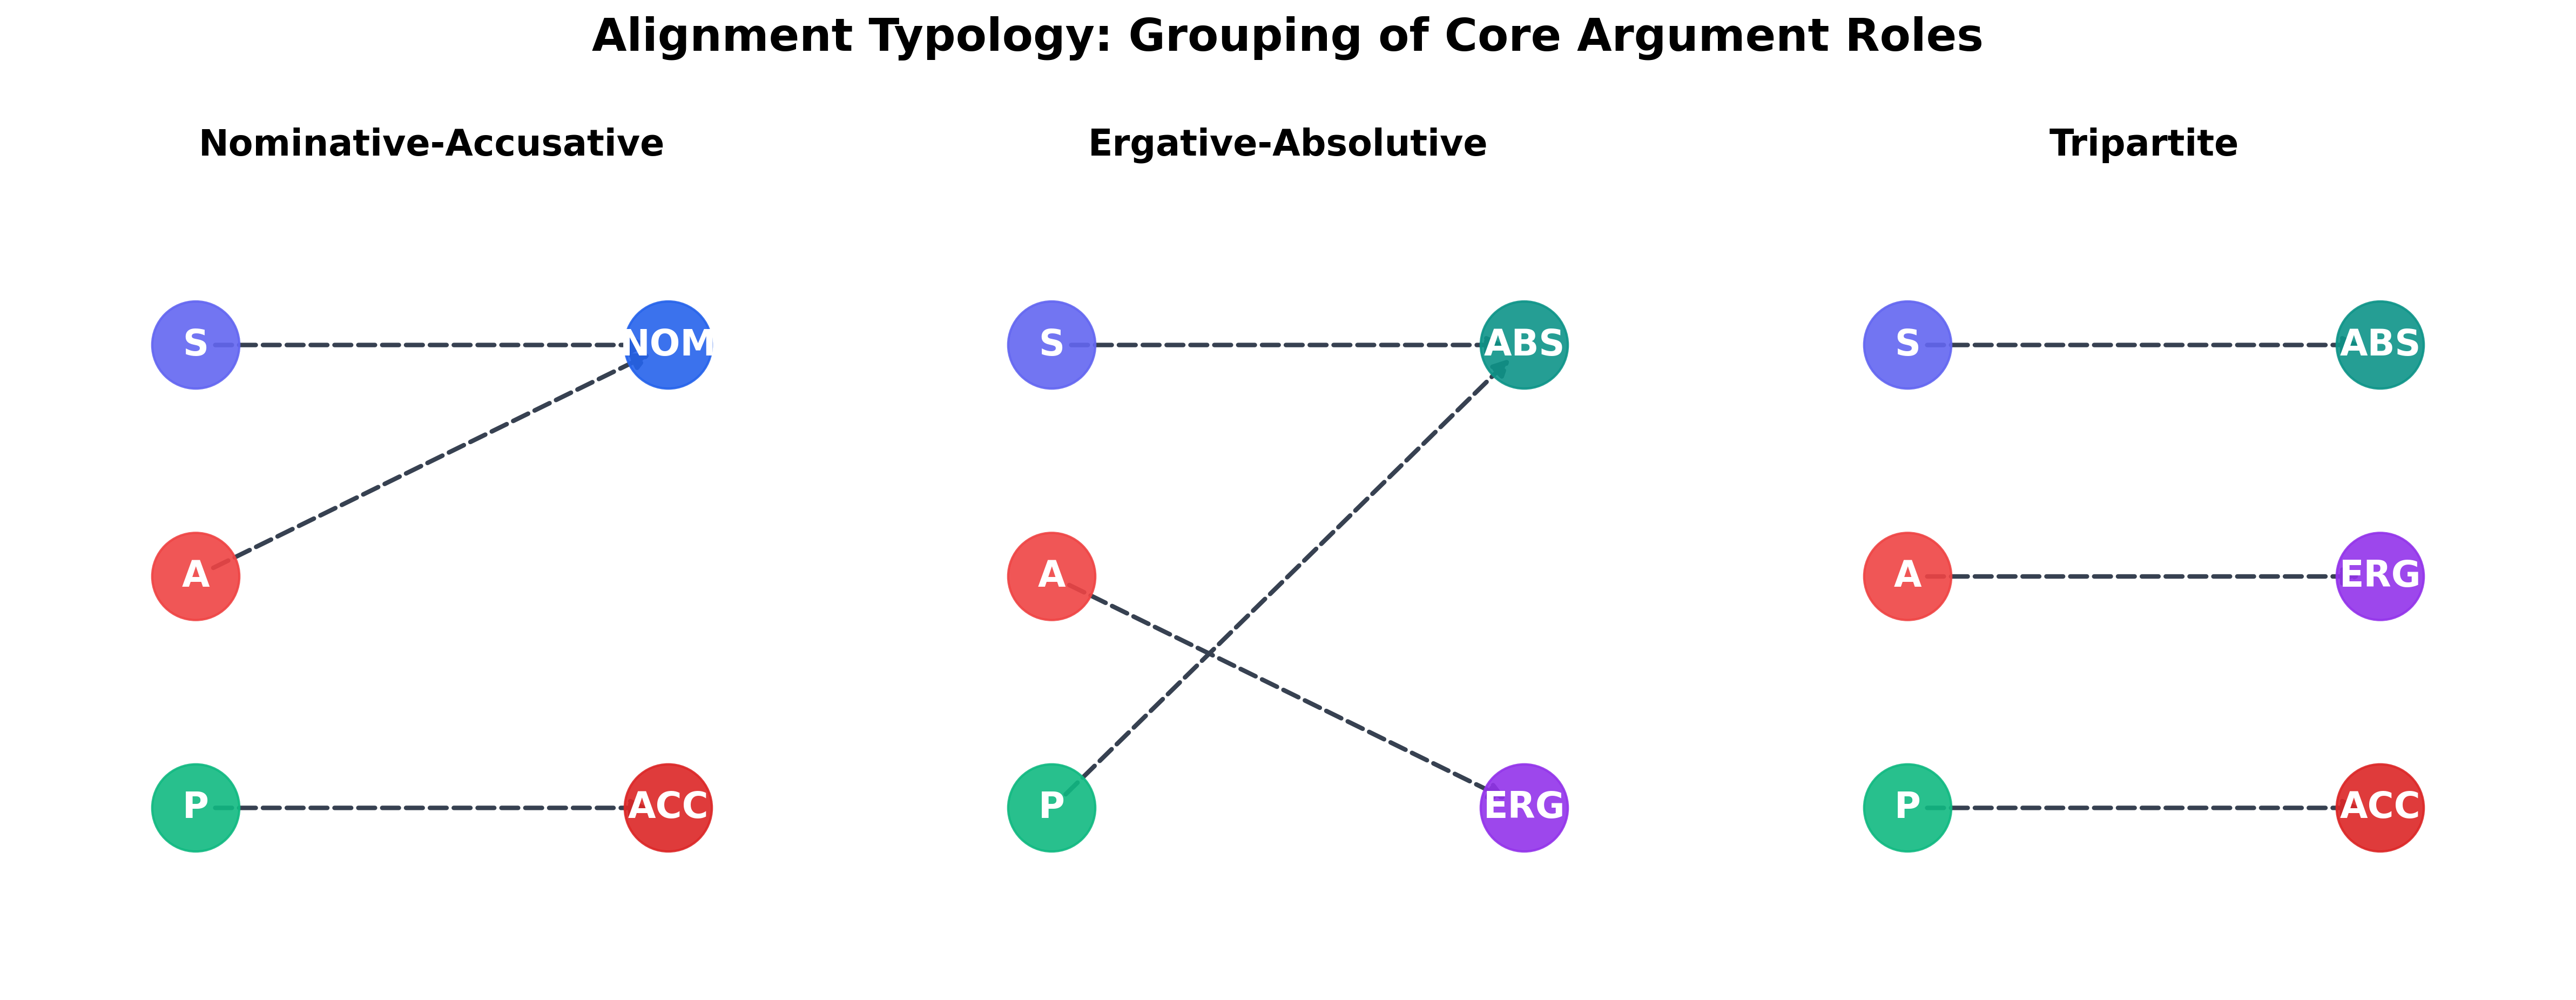
\includegraphics[keepaspectratio,alt={Functor kernels uniquely fingerprint each alignment typology. Three alignment systems realized as functors from \textbackslash mathcal\{U\} = \textbackslash\{S, A, P\textbackslash\}: Nominative--Accusative merges \textbackslash\{S,A\textbackslash\} \textbackslash to \textbackslash text\{NOM\} (kernel \textbackslash\{(S,A)\textbackslash\}, ); Ergative--Absolutive merges \textbackslash\{S,P\textbackslash\} \textbackslash to \textbackslash text\{ABS\} (kernel \textbackslash\{(S,P)\textbackslash\}, ); Tripartite is injective (kernel \textbackslash emptyset). Color-coded nodes reveal neutralization patterns: shared colors indicate functor identification of roles. Generated programmatically from the CaseCategory implementation.}]{../figures/alignment_comparison.png}}
\caption{Functor kernels uniquely fingerprint each alignment typology.
Three alignment systems realized as functors from
\(\mathcal{U} = \{S, A, P\}\): \textbf{Nominative--Accusative} merges
\(\{S,A\} \to \text{NOM}\) (kernel \(\{(S,A)\}\), \autoref{eq:eq-2-3});
\textbf{Ergative--Absolutive} merges \(\{S,P\} \to \text{ABS}\) (kernel
\(\{(S,P)\}\), \autoref{eq:eq-2-4}); \textbf{Tripartite} is injective
(kernel \(\emptyset\)). Color-coded nodes reveal neutralization
patterns: shared colors indicate functor identification of roles.
Generated programmatically from the \protect\texttt{CaseCategory}
implementation.}\label{fig:alignment}
\end{figure}

\begin{figure}
\centering
\pandocbounded{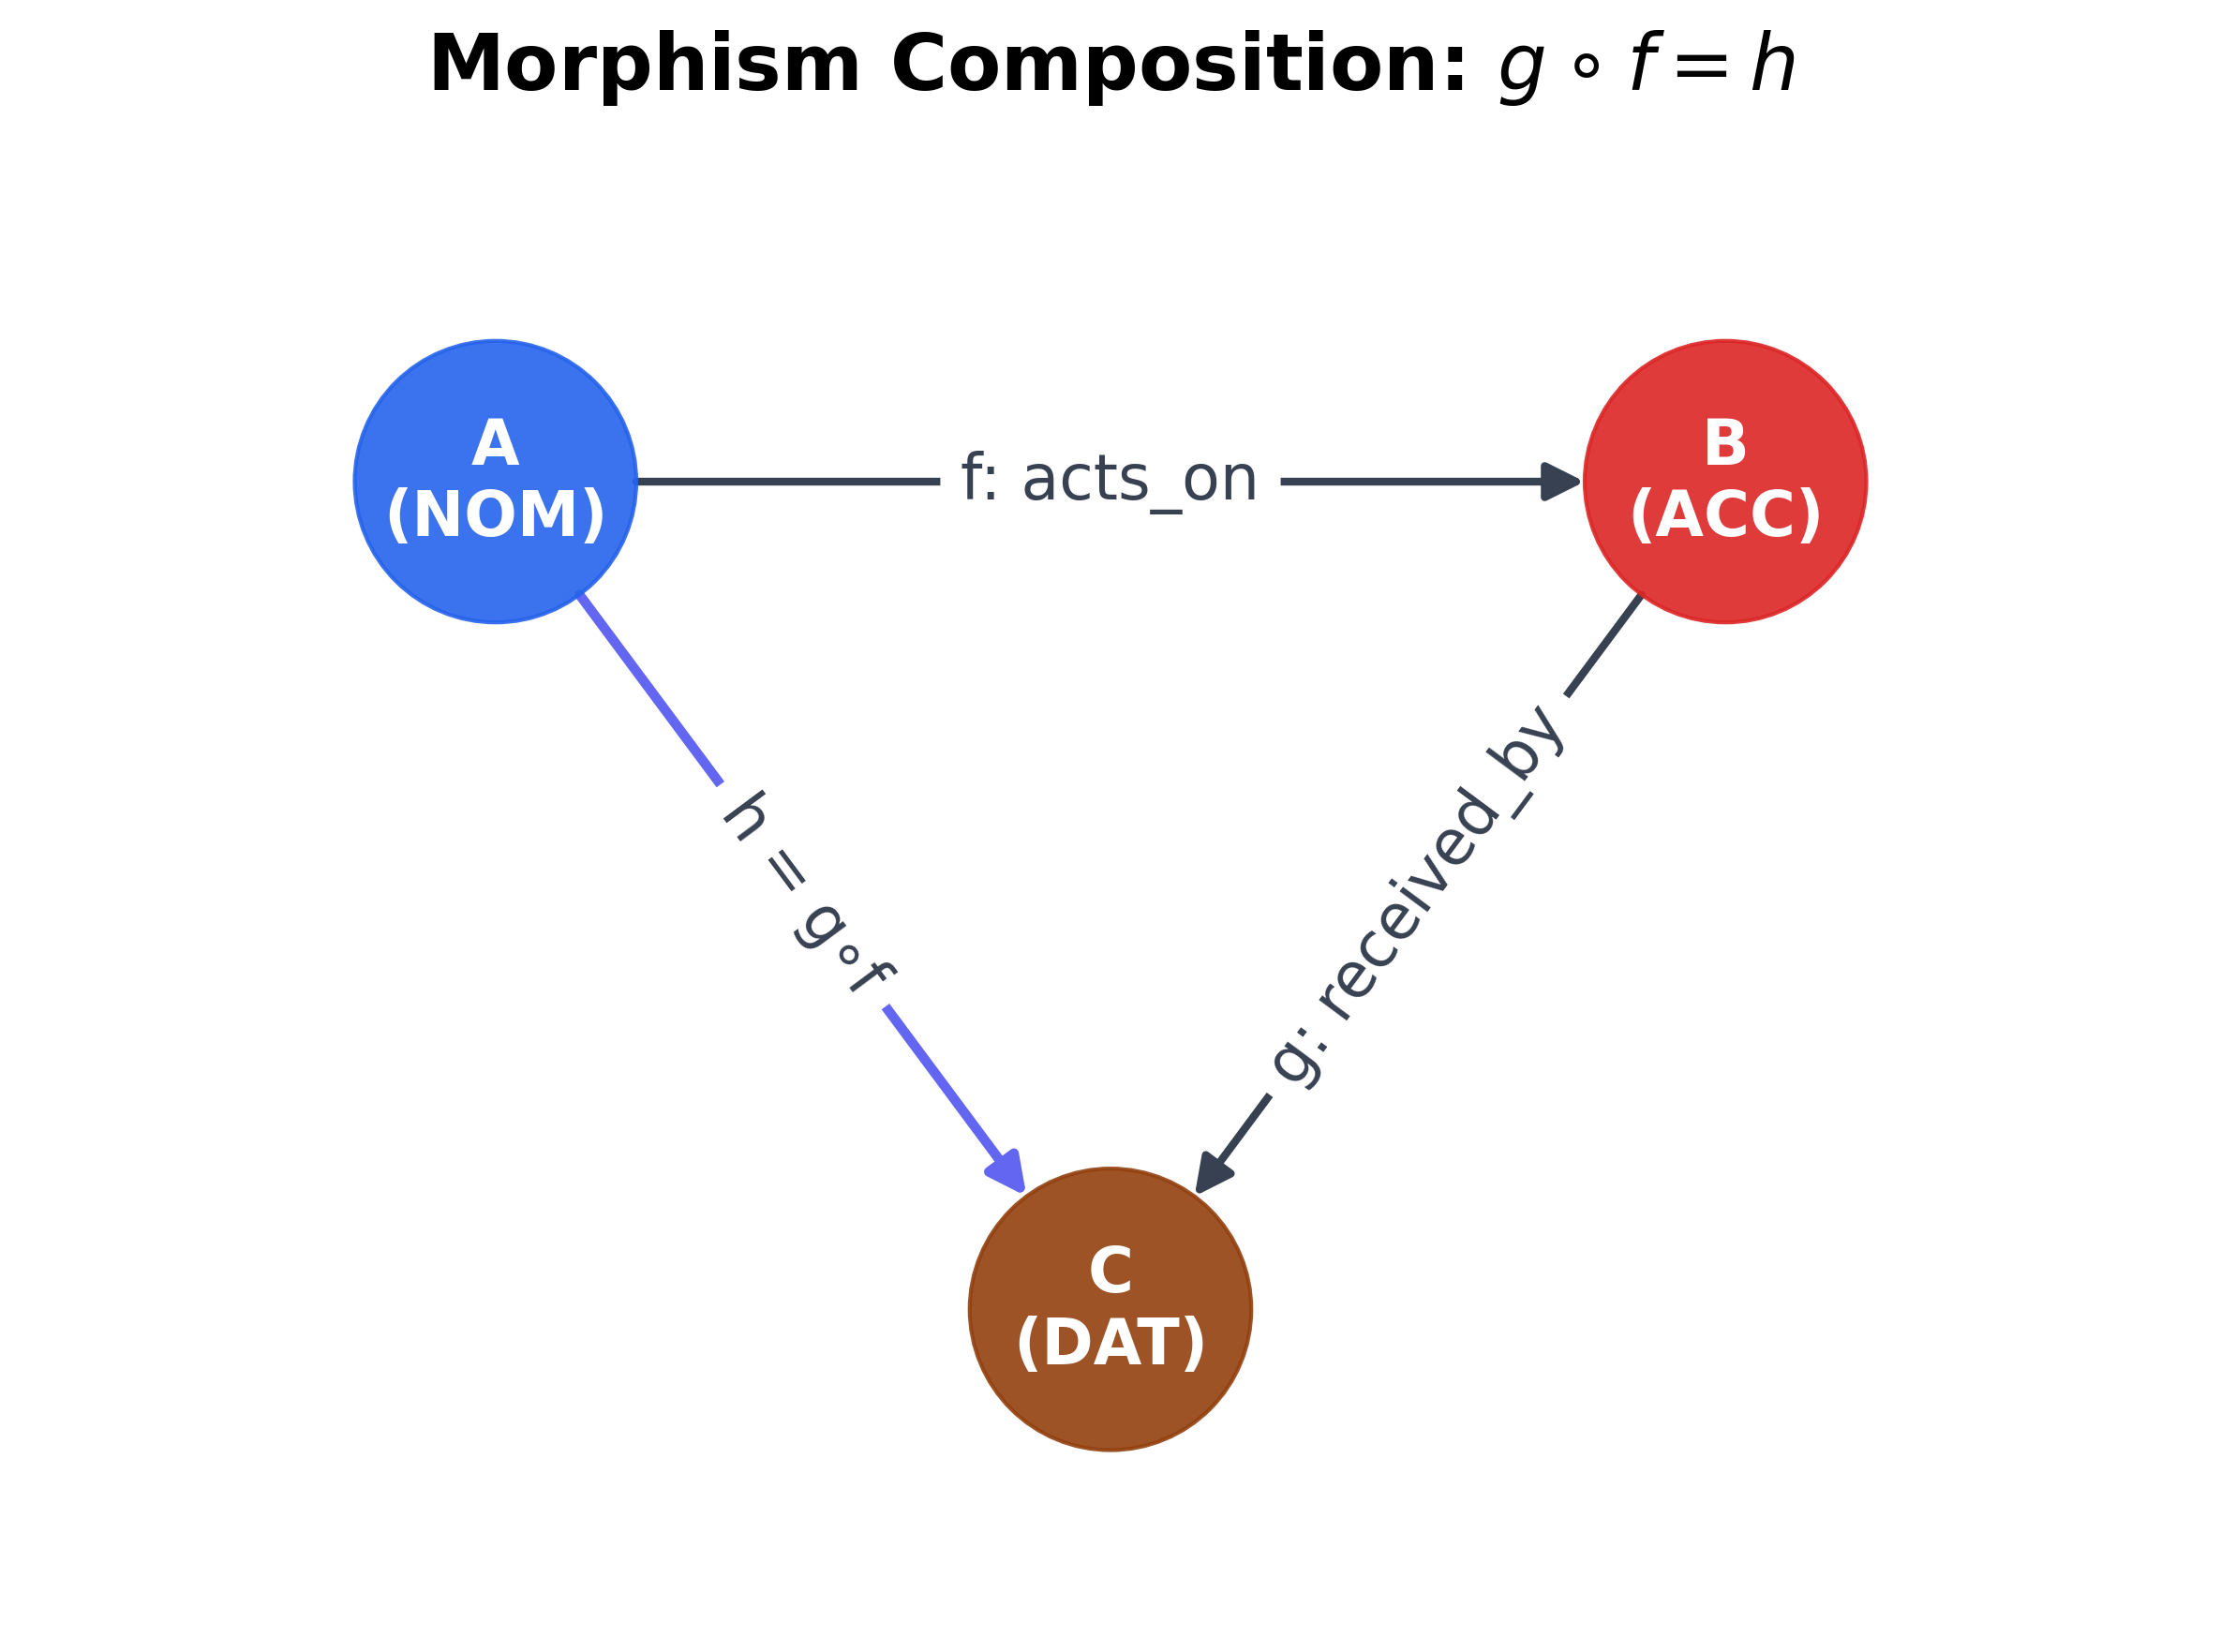
\includegraphics[keepaspectratio,alt={Morphism composition attenuates weights multiplicatively through intermediate case roles. Morphism f\textbackslash colon\textbackslash text\{NOM\}\textbackslash to\textbackslash text\{ACC\} (acts\_on) and g\textbackslash colon\textbackslash text\{ACC\}\textbackslash to\textbackslash text\{DAT\} (received\_by) compose to h = g \textbackslash circ f\textbackslash colon\textbackslash text\{NOM\}\textbackslash to\textbackslash text\{DAT\} per ; in the enriched category weights multiply (e.g., w\_f = 0.9, w\_g = 0.7 \textbackslash Rightarrow w(g \textbackslash circ f) = 0.63). The commutative triangle encodes that DAT assignment factors through ACC---the multiplicative attenuation reflects the typological observation that subject--recipient relations are weaker than the constituent subject--object and object--recipient links. Generated programmatically from the CaseCategory class.}]{../figures/composition_triangle.png}}
\caption{Morphism composition attenuates weights multiplicatively
through intermediate case roles. Morphism
\(f\colon\text{NOM}\to\text{ACC}\) (acts\_on) and
\(g\colon\text{ACC}\to\text{DAT}\) (received\_by) compose to
\(h = g \circ f\colon\text{NOM}\to\text{DAT}\) per \autoref{eq:eq-2-1};
in the enriched category weights multiply (e.g., \(w_f = 0.9\),
\(w_g = 0.7 \Rightarrow w(g \circ f) = 0.63\)). The commutative triangle
encodes that DAT assignment factors through ACC---the multiplicative
attenuation reflects the typological observation that subject--recipient
relations are weaker than the constituent subject--object and
object--recipient links. Generated programmatically from the
\protect\texttt{CaseCategory} class.}\label{fig:composition}
\end{figure}
\end{frame}

\begin{frame}[allowframebreaks]{Graded Proto-Roles as \([0,1]\)-Weighted
Morphisms}
\protect\phantomsection\label{graded-proto-roles-as-01-weighted-morphisms}
Following Dowty {[}-@dowty1991thematic{]}, we equip morphisms with
weights in \([0,1]\) that encode the degree of proto-role satisfaction.
A morphism \(f: \text{NOM} \to \text{ACC}\) with weight \(w = 0.9\)
indicates a strong transitive action (clear agent acting on clear
patient), while \(w = 0.4\) might indicate an experiencer construction
(``The child fears the dark'') where the nominative argument only weakly
satisfies Proto-Agent entailments.

\textbf{Slavic quirky case as overt evidence for sub-unit morphism
weights.} Russian and Serbian/BCS supply a sharper,
\emph{morphologically overt} witness for \(w < 1\): a class of verbs
that systematically refuses the canonical NOM \(\to\) ACC arrow and
instead routes its object through GEN, DAT, or INS. In Russian,
\emph{boyat'sja} ``to fear'' governs the genitive (\emph{boyus' sobaki}
``I fear the dog-GEN'', not *\emph{sobaku}-ACC); \emph{pomogat'} ``to
help'' governs the dative (\emph{pomogayu drugu} ``I help the
friend-DAT''); \emph{upravlyat'} ``to manage / steer'' governs the
instrumental (\emph{upravlyaet mašinoj} ``drives the car-INS'').
Serbian/BCS shows the same pattern: \emph{čestitati} ``to congratulate''
assigns DAT (\emph{čestitam prijatelju} ``I congratulate the
friend-DAT''); \emph{bojati se} ``to fear'' assigns GEN (\emph{bojim se
psa} ``I fear the dog-GEN''). Each such verb supplies an enriched
morphism whose target is \emph{not} ACC, equivalently a NOM \(\to\) ACC
arrow whose Dowtian weight has been reduced to near zero --- and the
reduction is visible in the suffix on the noun, not merely hypothesised
from semantics. These quirky-case lexemes are the cleanest empirical
anchor for the graded \([0,1]\)-enrichment we develop in
\autoref{sec:enriched-categories}.

Composition of enriched morphisms multiplies weights: \begin{equation}
w(g \circ f) = w(g) \cdot w(f)
\label{eq:eq-2-1}
\end{equation}

This multiplicative composition reflects the intuition that grammatical
dependencies attenuate as they chain through intermediate roles.
\autoref{fig:composition} illustrates the categorical composition of two
morphisms through an intermediate case role. The resulting structure is
a category enriched over \(([0,1], \cdot, 1)\)---a connection we develop
fully in \autoref{sec:enriched-categories}.
\end{frame}

\begin{frame}[fragile,allowframebreaks]{Alignment Shifts as Natural
Transformations: Functor Commutativity Encodes Grammar Agreement}
\protect\phantomsection\label{alignment-shifts-as-natural-transformations-functor-commutativity-encodes-grammar-agreement}
Having established that alignment systems are functors
\(F, G: \mathcal{U} \to \mathcal{L}\) from a universal case category to
language-specific categories, a natural question arises: \emph{how do
different alignment systems relate to each other?} The categorical
answer is a \textbf{natural transformation}
\(\alpha: F \Rightarrow G\)---a systematic family of morphisms
\(\alpha_A: F(A) \to G(A)\) for each case role \(A\), satisfying the
\textbf{naturality condition}:

\begin{equation}
G(f) \circ \alpha_A = \alpha_B \circ F(f) \quad \text{for every morphism } f: A \to B
\label{eq:eq-2-2}
\end{equation}

This naturality constraint is the formal expression of \emph{grammatical
coherence}: transforming one alignment into another and then applying a
grammatical relation yields the same result as first applying the
relation and then transforming---ensuring that alignment comparison
respects the relational fabric of the grammar.

\textbf{Worked example.} Consider the accusative functor \(F\) (which
maps S and A to NOM, P to ACC) alongside the tripartite functor \(G\)
(which maps explicitly to S \(\to\) ABS, A \(\to\) ERG, P \(\to\) ACC).
The \textbf{identity natural transformation}
\(\text{id}_F: F \Rightarrow F\) provides components
\({(\text{id}_F)}_A = \text{id}_{F{(A)}}\) over every role \(A\),
trivially satisfying the naturality condition. We construct the
\textbf{vertical composition} \(\beta \circ \alpha{}\) of two natural
transformations \(\alpha: F \Rightarrow G\) and
\(\beta: G \Rightarrow H\) purely componentwise:
\({(\beta \circ \alpha)}_A = \beta_A \circ \alpha_A\).

Our \texttt{NaturalTransformation} class implements these operations,
with \texttt{ComponentMorphism} objects encoding each \(\alpha_A\), and
\texttt{compose\_transformations()} implementing vertical composition.
The \texttt{IdentityNaturalTransformation} constructor automatically
generates identity components for every object in an
\texttt{AlignmentFunctor}'s domain. This machinery provides the formal
infrastructure for comparing alignment types not merely by listing their
neutralization patterns but by characterizing the \emph{structural
mappings} between them---e.g., the natural transformation from
accusative to tripartite alignment is injective (no two roles merge in
the target), while the transformation from tripartite to ergative is
non-injective (S and P merge into ABS).
\end{frame}

\end{document}
